\section{The Fibonacci Sequence}

\begin{figure}[h]
  \begin{center}
    % GNUPLOT: LaTeX picture
\setlength{\unitlength}{0.240900pt}
\ifx\plotpoint\undefined\newsavebox{\plotpoint}\fi
\sbox{\plotpoint}{\rule[-0.200pt]{0.400pt}{0.400pt}}%
\begin{picture}(1500,900)(0,0)
\sbox{\plotpoint}{\rule[-0.200pt]{0.400pt}{0.400pt}}%
\put(150.0,82.0){\rule[-0.200pt]{310.520pt}{0.400pt}}
\put(130,82){\makebox(0,0)[r]{ 0}}
\put(150.0,82.0){\rule[-0.200pt]{4.818pt}{0.400pt}}
\put(150.0,193.0){\rule[-0.200pt]{310.520pt}{0.400pt}}
\put(130,193){\makebox(0,0)[r]{ 1000}}
\put(150.0,193.0){\rule[-0.200pt]{4.818pt}{0.400pt}}
\put(150.0,304.0){\rule[-0.200pt]{310.520pt}{0.400pt}}
\put(130,304){\makebox(0,0)[r]{ 2000}}
\put(150.0,304.0){\rule[-0.200pt]{4.818pt}{0.400pt}}
\put(150.0,415.0){\rule[-0.200pt]{310.520pt}{0.400pt}}
\put(130,415){\makebox(0,0)[r]{ 3000}}
\put(150.0,415.0){\rule[-0.200pt]{4.818pt}{0.400pt}}
\put(150.0,526.0){\rule[-0.200pt]{310.520pt}{0.400pt}}
\put(130,526){\makebox(0,0)[r]{ 4000}}
\put(150.0,526.0){\rule[-0.200pt]{4.818pt}{0.400pt}}
\put(150.0,637.0){\rule[-0.200pt]{310.520pt}{0.400pt}}
\put(130,637){\makebox(0,0)[r]{ 5000}}
\put(150.0,637.0){\rule[-0.200pt]{4.818pt}{0.400pt}}
\put(150.0,748.0){\rule[-0.200pt]{310.520pt}{0.400pt}}
\put(130,748){\makebox(0,0)[r]{ 6000}}
\put(150.0,748.0){\rule[-0.200pt]{4.818pt}{0.400pt}}
\put(150.0,859.0){\rule[-0.200pt]{310.520pt}{0.400pt}}
\put(130,859){\makebox(0,0)[r]{ 7000}}
\put(150.0,859.0){\rule[-0.200pt]{4.818pt}{0.400pt}}
\put(150.0,82.0){\rule[-0.200pt]{0.400pt}{187.179pt}}
\put(150,41){\makebox(0,0){ 0}}
\put(150.0,82.0){\rule[-0.200pt]{0.400pt}{4.818pt}}
\put(472.0,82.0){\rule[-0.200pt]{0.400pt}{172.484pt}}
\put(472.0,839.0){\rule[-0.200pt]{0.400pt}{4.818pt}}
\put(472,41){\makebox(0,0){ 5}}
\put(472.0,82.0){\rule[-0.200pt]{0.400pt}{4.818pt}}
\put(795.0,82.0){\rule[-0.200pt]{0.400pt}{187.179pt}}
\put(795,41){\makebox(0,0){ 10}}
\put(795.0,82.0){\rule[-0.200pt]{0.400pt}{4.818pt}}
\put(1117.0,82.0){\rule[-0.200pt]{0.400pt}{187.179pt}}
\put(1117,41){\makebox(0,0){ 15}}
\put(1117.0,82.0){\rule[-0.200pt]{0.400pt}{4.818pt}}
\put(1439.0,82.0){\rule[-0.200pt]{0.400pt}{187.179pt}}
\put(1439,41){\makebox(0,0){ 20}}
\put(1439.0,82.0){\rule[-0.200pt]{0.400pt}{4.818pt}}
\put(150.0,82.0){\rule[-0.200pt]{0.400pt}{187.179pt}}
\put(150.0,82.0){\rule[-0.200pt]{310.520pt}{0.400pt}}
\put(530,819){\makebox(0,0)[r]{\(F_n\)}}
\put(550.0,819.0){\rule[-0.200pt]{24.090pt}{0.400pt}}
\put(150,82){\usebox{\plotpoint}}
\put(472,81.67){\rule{0.482pt}{0.400pt}}
\multiput(472.00,81.17)(1.000,1.000){2}{\rule{0.241pt}{0.400pt}}
\put(150.0,82.0){\rule[-0.200pt]{77.570pt}{0.400pt}}
\put(610,82.67){\rule{0.241pt}{0.400pt}}
\multiput(610.00,82.17)(0.500,1.000){2}{\rule{0.120pt}{0.400pt}}
\put(474.0,83.0){\rule[-0.200pt]{32.762pt}{0.400pt}}
\put(677,83.67){\rule{0.241pt}{0.400pt}}
\multiput(677.00,83.17)(0.500,1.000){2}{\rule{0.120pt}{0.400pt}}
\put(611.0,84.0){\rule[-0.200pt]{15.899pt}{0.400pt}}
\put(721,84.67){\rule{0.241pt}{0.400pt}}
\multiput(721.00,84.17)(0.500,1.000){2}{\rule{0.120pt}{0.400pt}}
\put(678.0,85.0){\rule[-0.200pt]{10.359pt}{0.400pt}}
\put(755,85.67){\rule{0.241pt}{0.400pt}}
\multiput(755.00,85.17)(0.500,1.000){2}{\rule{0.120pt}{0.400pt}}
\put(722.0,86.0){\rule[-0.200pt]{7.950pt}{0.400pt}}
\put(782,86.67){\rule{0.241pt}{0.400pt}}
\multiput(782.00,86.17)(0.500,1.000){2}{\rule{0.120pt}{0.400pt}}
\put(756.0,87.0){\rule[-0.200pt]{6.263pt}{0.400pt}}
\put(804,87.67){\rule{0.241pt}{0.400pt}}
\multiput(804.00,87.17)(0.500,1.000){2}{\rule{0.120pt}{0.400pt}}
\put(783.0,88.0){\rule[-0.200pt]{5.059pt}{0.400pt}}
\put(823,88.67){\rule{0.241pt}{0.400pt}}
\multiput(823.00,88.17)(0.500,1.000){2}{\rule{0.120pt}{0.400pt}}
\put(805.0,89.0){\rule[-0.200pt]{4.336pt}{0.400pt}}
\put(838,89.67){\rule{0.482pt}{0.400pt}}
\multiput(838.00,89.17)(1.000,1.000){2}{\rule{0.241pt}{0.400pt}}
\put(824.0,90.0){\rule[-0.200pt]{3.373pt}{0.400pt}}
\put(854,90.67){\rule{0.241pt}{0.400pt}}
\multiput(854.00,90.17)(0.500,1.000){2}{\rule{0.120pt}{0.400pt}}
\put(840.0,91.0){\rule[-0.200pt]{3.373pt}{0.400pt}}
\put(867,91.67){\rule{0.241pt}{0.400pt}}
\multiput(867.00,91.17)(0.500,1.000){2}{\rule{0.120pt}{0.400pt}}
\put(855.0,92.0){\rule[-0.200pt]{2.891pt}{0.400pt}}
\put(880,92.67){\rule{0.241pt}{0.400pt}}
\multiput(880.00,92.17)(0.500,1.000){2}{\rule{0.120pt}{0.400pt}}
\put(868.0,93.0){\rule[-0.200pt]{2.891pt}{0.400pt}}
\put(890,93.67){\rule{0.241pt}{0.400pt}}
\multiput(890.00,93.17)(0.500,1.000){2}{\rule{0.120pt}{0.400pt}}
\put(881.0,94.0){\rule[-0.200pt]{2.168pt}{0.400pt}}
\put(900,94.67){\rule{0.241pt}{0.400pt}}
\multiput(900.00,94.17)(0.500,1.000){2}{\rule{0.120pt}{0.400pt}}
\put(891.0,95.0){\rule[-0.200pt]{2.168pt}{0.400pt}}
\put(911,95.67){\rule{0.241pt}{0.400pt}}
\multiput(911.00,95.17)(0.500,1.000){2}{\rule{0.120pt}{0.400pt}}
\put(901.0,96.0){\rule[-0.200pt]{2.409pt}{0.400pt}}
\put(920,96.67){\rule{0.241pt}{0.400pt}}
\multiput(920.00,96.17)(0.500,1.000){2}{\rule{0.120pt}{0.400pt}}
\put(912.0,97.0){\rule[-0.200pt]{1.927pt}{0.400pt}}
\put(927,97.67){\rule{0.482pt}{0.400pt}}
\multiput(927.00,97.17)(1.000,1.000){2}{\rule{0.241pt}{0.400pt}}
\put(921.0,98.0){\rule[-0.200pt]{1.445pt}{0.400pt}}
\put(935,98.67){\rule{0.241pt}{0.400pt}}
\multiput(935.00,98.17)(0.500,1.000){2}{\rule{0.120pt}{0.400pt}}
\put(929.0,99.0){\rule[-0.200pt]{1.445pt}{0.400pt}}
\put(943,99.67){\rule{0.241pt}{0.400pt}}
\multiput(943.00,99.17)(0.500,1.000){2}{\rule{0.120pt}{0.400pt}}
\put(936.0,100.0){\rule[-0.200pt]{1.686pt}{0.400pt}}
\put(949,100.67){\rule{0.241pt}{0.400pt}}
\multiput(949.00,100.17)(0.500,1.000){2}{\rule{0.120pt}{0.400pt}}
\put(944.0,101.0){\rule[-0.200pt]{1.204pt}{0.400pt}}
\put(957,101.67){\rule{0.241pt}{0.400pt}}
\multiput(957.00,101.17)(0.500,1.000){2}{\rule{0.120pt}{0.400pt}}
\put(950.0,102.0){\rule[-0.200pt]{1.686pt}{0.400pt}}
\put(962,102.67){\rule{0.241pt}{0.400pt}}
\multiput(962.00,102.17)(0.500,1.000){2}{\rule{0.120pt}{0.400pt}}
\put(958.0,103.0){\rule[-0.200pt]{0.964pt}{0.400pt}}
\put(969,103.67){\rule{0.241pt}{0.400pt}}
\multiput(969.00,103.17)(0.500,1.000){2}{\rule{0.120pt}{0.400pt}}
\put(963.0,104.0){\rule[-0.200pt]{1.445pt}{0.400pt}}
\put(975,104.67){\rule{0.241pt}{0.400pt}}
\multiput(975.00,104.17)(0.500,1.000){2}{\rule{0.120pt}{0.400pt}}
\put(970.0,105.0){\rule[-0.200pt]{1.204pt}{0.400pt}}
\put(980,105.67){\rule{0.241pt}{0.400pt}}
\multiput(980.00,105.17)(0.500,1.000){2}{\rule{0.120pt}{0.400pt}}
\put(976.0,106.0){\rule[-0.200pt]{0.964pt}{0.400pt}}
\put(985,106.67){\rule{0.482pt}{0.400pt}}
\multiput(985.00,106.17)(1.000,1.000){2}{\rule{0.241pt}{0.400pt}}
\put(981.0,107.0){\rule[-0.200pt]{0.964pt}{0.400pt}}
\put(990,107.67){\rule{0.482pt}{0.400pt}}
\multiput(990.00,107.17)(1.000,1.000){2}{\rule{0.241pt}{0.400pt}}
\put(987.0,108.0){\rule[-0.200pt]{0.723pt}{0.400pt}}
\put(996,108.67){\rule{0.241pt}{0.400pt}}
\multiput(996.00,108.17)(0.500,1.000){2}{\rule{0.120pt}{0.400pt}}
\put(992.0,109.0){\rule[-0.200pt]{0.964pt}{0.400pt}}
\put(1001,109.67){\rule{0.241pt}{0.400pt}}
\multiput(1001.00,109.17)(0.500,1.000){2}{\rule{0.120pt}{0.400pt}}
\put(997.0,110.0){\rule[-0.200pt]{0.964pt}{0.400pt}}
\put(1005,110.67){\rule{0.241pt}{0.400pt}}
\multiput(1005.00,110.17)(0.500,1.000){2}{\rule{0.120pt}{0.400pt}}
\put(1002.0,111.0){\rule[-0.200pt]{0.723pt}{0.400pt}}
\put(1010,111.67){\rule{0.241pt}{0.400pt}}
\multiput(1010.00,111.17)(0.500,1.000){2}{\rule{0.120pt}{0.400pt}}
\put(1006.0,112.0){\rule[-0.200pt]{0.964pt}{0.400pt}}
\put(1014,112.67){\rule{0.241pt}{0.400pt}}
\multiput(1014.00,112.17)(0.500,1.000){2}{\rule{0.120pt}{0.400pt}}
\put(1011.0,113.0){\rule[-0.200pt]{0.723pt}{0.400pt}}
\put(1017,113.67){\rule{0.482pt}{0.400pt}}
\multiput(1017.00,113.17)(1.000,1.000){2}{\rule{0.241pt}{0.400pt}}
\put(1015.0,114.0){\rule[-0.200pt]{0.482pt}{0.400pt}}
\put(1021,114.67){\rule{0.482pt}{0.400pt}}
\multiput(1021.00,114.17)(1.000,1.000){2}{\rule{0.241pt}{0.400pt}}
\put(1019.0,115.0){\rule[-0.200pt]{0.482pt}{0.400pt}}
\put(1027,115.67){\rule{0.241pt}{0.400pt}}
\multiput(1027.00,115.17)(0.500,1.000){2}{\rule{0.120pt}{0.400pt}}
\put(1023.0,116.0){\rule[-0.200pt]{0.964pt}{0.400pt}}
\put(1029,116.67){\rule{0.241pt}{0.400pt}}
\multiput(1029.00,116.17)(0.500,1.000){2}{\rule{0.120pt}{0.400pt}}
\put(1028.0,117.0){\usebox{\plotpoint}}
\put(1033,117.67){\rule{0.241pt}{0.400pt}}
\multiput(1033.00,117.17)(0.500,1.000){2}{\rule{0.120pt}{0.400pt}}
\put(1030.0,118.0){\rule[-0.200pt]{0.723pt}{0.400pt}}
\put(1037,118.67){\rule{0.241pt}{0.400pt}}
\multiput(1037.00,118.17)(0.500,1.000){2}{\rule{0.120pt}{0.400pt}}
\put(1034.0,119.0){\rule[-0.200pt]{0.723pt}{0.400pt}}
\put(1041,119.67){\rule{0.241pt}{0.400pt}}
\multiput(1041.00,119.17)(0.500,1.000){2}{\rule{0.120pt}{0.400pt}}
\put(1038.0,120.0){\rule[-0.200pt]{0.723pt}{0.400pt}}
\put(1045,120.67){\rule{0.241pt}{0.400pt}}
\multiput(1045.00,120.17)(0.500,1.000){2}{\rule{0.120pt}{0.400pt}}
\put(1042.0,121.0){\rule[-0.200pt]{0.723pt}{0.400pt}}
\put(1047,121.67){\rule{0.241pt}{0.400pt}}
\multiput(1047.00,121.17)(0.500,1.000){2}{\rule{0.120pt}{0.400pt}}
\put(1046.0,122.0){\usebox{\plotpoint}}
\put(1051,122.67){\rule{0.241pt}{0.400pt}}
\multiput(1051.00,122.17)(0.500,1.000){2}{\rule{0.120pt}{0.400pt}}
\put(1048.0,123.0){\rule[-0.200pt]{0.723pt}{0.400pt}}
\put(1054,123.67){\rule{0.241pt}{0.400pt}}
\multiput(1054.00,123.17)(0.500,1.000){2}{\rule{0.120pt}{0.400pt}}
\put(1052.0,124.0){\rule[-0.200pt]{0.482pt}{0.400pt}}
\put(1057,124.67){\rule{0.482pt}{0.400pt}}
\multiput(1057.00,124.17)(1.000,1.000){2}{\rule{0.241pt}{0.400pt}}
\put(1055.0,125.0){\rule[-0.200pt]{0.482pt}{0.400pt}}
\put(1060,125.67){\rule{0.241pt}{0.400pt}}
\multiput(1060.00,125.17)(0.500,1.000){2}{\rule{0.120pt}{0.400pt}}
\put(1059.0,126.0){\usebox{\plotpoint}}
\put(1063,126.67){\rule{0.241pt}{0.400pt}}
\multiput(1063.00,126.17)(0.500,1.000){2}{\rule{0.120pt}{0.400pt}}
\put(1061.0,127.0){\rule[-0.200pt]{0.482pt}{0.400pt}}
\put(1065,127.67){\rule{0.241pt}{0.400pt}}
\multiput(1065.00,127.17)(0.500,1.000){2}{\rule{0.120pt}{0.400pt}}
\put(1064.0,128.0){\usebox{\plotpoint}}
\put(1069,128.67){\rule{0.241pt}{0.400pt}}
\multiput(1069.00,128.17)(0.500,1.000){2}{\rule{0.120pt}{0.400pt}}
\put(1066.0,129.0){\rule[-0.200pt]{0.723pt}{0.400pt}}
\put(1072,129.67){\rule{0.241pt}{0.400pt}}
\multiput(1072.00,129.17)(0.500,1.000){2}{\rule{0.120pt}{0.400pt}}
\put(1070.0,130.0){\rule[-0.200pt]{0.482pt}{0.400pt}}
\put(1074,130.67){\rule{0.482pt}{0.400pt}}
\multiput(1074.00,130.17)(1.000,1.000){2}{\rule{0.241pt}{0.400pt}}
\put(1073.0,131.0){\usebox{\plotpoint}}
\put(1077,131.67){\rule{0.241pt}{0.400pt}}
\multiput(1077.00,131.17)(0.500,1.000){2}{\rule{0.120pt}{0.400pt}}
\put(1076.0,132.0){\usebox{\plotpoint}}
\put(1079,132.67){\rule{0.482pt}{0.400pt}}
\multiput(1079.00,132.17)(1.000,1.000){2}{\rule{0.241pt}{0.400pt}}
\put(1078.0,133.0){\usebox{\plotpoint}}
\put(1082,133.67){\rule{0.241pt}{0.400pt}}
\multiput(1082.00,133.17)(0.500,1.000){2}{\rule{0.120pt}{0.400pt}}
\put(1081.0,134.0){\usebox{\plotpoint}}
\put(1085,134.67){\rule{0.241pt}{0.400pt}}
\multiput(1085.00,134.17)(0.500,1.000){2}{\rule{0.120pt}{0.400pt}}
\put(1083.0,135.0){\rule[-0.200pt]{0.482pt}{0.400pt}}
\put(1087,135.67){\rule{0.241pt}{0.400pt}}
\multiput(1087.00,135.17)(0.500,1.000){2}{\rule{0.120pt}{0.400pt}}
\put(1086.0,136.0){\usebox{\plotpoint}}
\put(1090,136.67){\rule{0.241pt}{0.400pt}}
\multiput(1090.00,136.17)(0.500,1.000){2}{\rule{0.120pt}{0.400pt}}
\put(1088.0,137.0){\rule[-0.200pt]{0.482pt}{0.400pt}}
\put(1092,137.67){\rule{0.482pt}{0.400pt}}
\multiput(1092.00,137.17)(1.000,1.000){2}{\rule{0.241pt}{0.400pt}}
\put(1091.0,138.0){\usebox{\plotpoint}}
\put(1095,138.67){\rule{0.241pt}{0.400pt}}
\multiput(1095.00,138.17)(0.500,1.000){2}{\rule{0.120pt}{0.400pt}}
\put(1094.0,139.0){\usebox{\plotpoint}}
\put(1097,139.67){\rule{0.482pt}{0.400pt}}
\multiput(1097.00,139.17)(1.000,1.000){2}{\rule{0.241pt}{0.400pt}}
\put(1099,140.67){\rule{0.241pt}{0.400pt}}
\multiput(1099.00,140.17)(0.500,1.000){2}{\rule{0.120pt}{0.400pt}}
\put(1096.0,140.0){\usebox{\plotpoint}}
\put(1101,141.67){\rule{0.482pt}{0.400pt}}
\multiput(1101.00,141.17)(1.000,1.000){2}{\rule{0.241pt}{0.400pt}}
\put(1100.0,142.0){\usebox{\plotpoint}}
\put(1104,142.67){\rule{0.241pt}{0.400pt}}
\multiput(1104.00,142.17)(0.500,1.000){2}{\rule{0.120pt}{0.400pt}}
\put(1105,143.67){\rule{0.241pt}{0.400pt}}
\multiput(1105.00,143.17)(0.500,1.000){2}{\rule{0.120pt}{0.400pt}}
\put(1103.0,143.0){\usebox{\plotpoint}}
\put(1108,144.67){\rule{0.241pt}{0.400pt}}
\multiput(1108.00,144.17)(0.500,1.000){2}{\rule{0.120pt}{0.400pt}}
\put(1106.0,145.0){\rule[-0.200pt]{0.482pt}{0.400pt}}
\put(1110,145.67){\rule{0.482pt}{0.400pt}}
\multiput(1110.00,145.17)(1.000,1.000){2}{\rule{0.241pt}{0.400pt}}
\put(1112,146.67){\rule{0.241pt}{0.400pt}}
\multiput(1112.00,146.17)(0.500,1.000){2}{\rule{0.120pt}{0.400pt}}
\put(1109.0,146.0){\usebox{\plotpoint}}
\put(1114,147.67){\rule{0.241pt}{0.400pt}}
\multiput(1114.00,147.17)(0.500,1.000){2}{\rule{0.120pt}{0.400pt}}
\put(1115,148.67){\rule{0.482pt}{0.400pt}}
\multiput(1115.00,148.17)(1.000,1.000){2}{\rule{0.241pt}{0.400pt}}
\put(1113.0,148.0){\usebox{\plotpoint}}
\put(1118,149.67){\rule{0.241pt}{0.400pt}}
\multiput(1118.00,149.17)(0.500,1.000){2}{\rule{0.120pt}{0.400pt}}
\put(1119,150.67){\rule{0.482pt}{0.400pt}}
\multiput(1119.00,150.17)(1.000,1.000){2}{\rule{0.241pt}{0.400pt}}
\put(1117.0,150.0){\usebox{\plotpoint}}
\put(1122,151.67){\rule{0.241pt}{0.400pt}}
\multiput(1122.00,151.17)(0.500,1.000){2}{\rule{0.120pt}{0.400pt}}
\put(1123,152.67){\rule{0.241pt}{0.400pt}}
\multiput(1123.00,152.17)(0.500,1.000){2}{\rule{0.120pt}{0.400pt}}
\put(1121.0,152.0){\usebox{\plotpoint}}
\put(1126,153.67){\rule{0.241pt}{0.400pt}}
\multiput(1126.00,153.17)(0.500,1.000){2}{\rule{0.120pt}{0.400pt}}
\put(1127,154.67){\rule{0.241pt}{0.400pt}}
\multiput(1127.00,154.17)(0.500,1.000){2}{\rule{0.120pt}{0.400pt}}
\put(1124.0,154.0){\rule[-0.200pt]{0.482pt}{0.400pt}}
\put(1130,155.67){\rule{0.241pt}{0.400pt}}
\multiput(1130.00,155.17)(0.500,1.000){2}{\rule{0.120pt}{0.400pt}}
\put(1131,156.67){\rule{0.241pt}{0.400pt}}
\multiput(1131.00,156.17)(0.500,1.000){2}{\rule{0.120pt}{0.400pt}}
\put(1132,157.67){\rule{0.482pt}{0.400pt}}
\multiput(1132.00,157.17)(1.000,1.000){2}{\rule{0.241pt}{0.400pt}}
\put(1128.0,156.0){\rule[-0.200pt]{0.482pt}{0.400pt}}
\put(1135,158.67){\rule{0.241pt}{0.400pt}}
\multiput(1135.00,158.17)(0.500,1.000){2}{\rule{0.120pt}{0.400pt}}
\put(1136,159.67){\rule{0.241pt}{0.400pt}}
\multiput(1136.00,159.17)(0.500,1.000){2}{\rule{0.120pt}{0.400pt}}
\put(1137,160.67){\rule{0.482pt}{0.400pt}}
\multiput(1137.00,160.17)(1.000,1.000){2}{\rule{0.241pt}{0.400pt}}
\put(1134.0,159.0){\usebox{\plotpoint}}
\put(1140,161.67){\rule{0.241pt}{0.400pt}}
\multiput(1140.00,161.17)(0.500,1.000){2}{\rule{0.120pt}{0.400pt}}
\put(1141,162.67){\rule{0.482pt}{0.400pt}}
\multiput(1141.00,162.17)(1.000,1.000){2}{\rule{0.241pt}{0.400pt}}
\put(1143,163.67){\rule{0.241pt}{0.400pt}}
\multiput(1143.00,163.17)(0.500,1.000){2}{\rule{0.120pt}{0.400pt}}
\put(1144,164.67){\rule{0.241pt}{0.400pt}}
\multiput(1144.00,164.17)(0.500,1.000){2}{\rule{0.120pt}{0.400pt}}
\put(1139.0,162.0){\usebox{\plotpoint}}
\put(1146,165.67){\rule{0.482pt}{0.400pt}}
\multiput(1146.00,165.17)(1.000,1.000){2}{\rule{0.241pt}{0.400pt}}
\put(1148,166.67){\rule{0.241pt}{0.400pt}}
\multiput(1148.00,166.17)(0.500,1.000){2}{\rule{0.120pt}{0.400pt}}
\put(1149,167.67){\rule{0.241pt}{0.400pt}}
\multiput(1149.00,167.17)(0.500,1.000){2}{\rule{0.120pt}{0.400pt}}
\put(1150,168.67){\rule{0.482pt}{0.400pt}}
\multiput(1150.00,168.17)(1.000,1.000){2}{\rule{0.241pt}{0.400pt}}
\put(1152,169.67){\rule{0.241pt}{0.400pt}}
\multiput(1152.00,169.17)(0.500,1.000){2}{\rule{0.120pt}{0.400pt}}
\put(1145.0,166.0){\usebox{\plotpoint}}
\put(1154,170.67){\rule{0.241pt}{0.400pt}}
\multiput(1154.00,170.17)(0.500,1.000){2}{\rule{0.120pt}{0.400pt}}
\put(1155,171.67){\rule{0.482pt}{0.400pt}}
\multiput(1155.00,171.17)(1.000,1.000){2}{\rule{0.241pt}{0.400pt}}
\put(1157,172.67){\rule{0.241pt}{0.400pt}}
\multiput(1157.00,172.17)(0.500,1.000){2}{\rule{0.120pt}{0.400pt}}
\put(1158,173.67){\rule{0.241pt}{0.400pt}}
\multiput(1158.00,173.17)(0.500,1.000){2}{\rule{0.120pt}{0.400pt}}
\put(1159,174.67){\rule{0.482pt}{0.400pt}}
\multiput(1159.00,174.17)(1.000,1.000){2}{\rule{0.241pt}{0.400pt}}
\put(1161,175.67){\rule{0.241pt}{0.400pt}}
\multiput(1161.00,175.17)(0.500,1.000){2}{\rule{0.120pt}{0.400pt}}
\put(1162,176.67){\rule{0.241pt}{0.400pt}}
\multiput(1162.00,176.17)(0.500,1.000){2}{\rule{0.120pt}{0.400pt}}
\put(1163,177.67){\rule{0.241pt}{0.400pt}}
\multiput(1163.00,177.17)(0.500,1.000){2}{\rule{0.120pt}{0.400pt}}
\put(1164,178.67){\rule{0.482pt}{0.400pt}}
\multiput(1164.00,178.17)(1.000,1.000){2}{\rule{0.241pt}{0.400pt}}
\put(1153.0,171.0){\usebox{\plotpoint}}
\put(1167,179.67){\rule{0.241pt}{0.400pt}}
\multiput(1167.00,179.17)(0.500,1.000){2}{\rule{0.120pt}{0.400pt}}
\put(1168,180.67){\rule{0.482pt}{0.400pt}}
\multiput(1168.00,180.17)(1.000,1.000){2}{\rule{0.241pt}{0.400pt}}
\put(1170,181.67){\rule{0.241pt}{0.400pt}}
\multiput(1170.00,181.17)(0.500,1.000){2}{\rule{0.120pt}{0.400pt}}
\put(1171,182.67){\rule{0.241pt}{0.400pt}}
\multiput(1171.00,182.17)(0.500,1.000){2}{\rule{0.120pt}{0.400pt}}
\put(1172,183.67){\rule{0.241pt}{0.400pt}}
\multiput(1172.00,183.17)(0.500,1.000){2}{\rule{0.120pt}{0.400pt}}
\put(1173,184.67){\rule{0.482pt}{0.400pt}}
\multiput(1173.00,184.17)(1.000,1.000){2}{\rule{0.241pt}{0.400pt}}
\put(1175,185.67){\rule{0.241pt}{0.400pt}}
\multiput(1175.00,185.17)(0.500,1.000){2}{\rule{0.120pt}{0.400pt}}
\put(1176,186.67){\rule{0.241pt}{0.400pt}}
\multiput(1176.00,186.17)(0.500,1.000){2}{\rule{0.120pt}{0.400pt}}
\put(1177,187.67){\rule{0.482pt}{0.400pt}}
\multiput(1177.00,187.17)(1.000,1.000){2}{\rule{0.241pt}{0.400pt}}
\put(1179,188.67){\rule{0.241pt}{0.400pt}}
\multiput(1179.00,188.17)(0.500,1.000){2}{\rule{0.120pt}{0.400pt}}
\put(1179.67,190){\rule{0.400pt}{0.482pt}}
\multiput(1179.17,190.00)(1.000,1.000){2}{\rule{0.400pt}{0.241pt}}
\put(1181,191.67){\rule{0.241pt}{0.400pt}}
\multiput(1181.00,191.17)(0.500,1.000){2}{\rule{0.120pt}{0.400pt}}
\put(1182,192.67){\rule{0.482pt}{0.400pt}}
\multiput(1182.00,192.17)(1.000,1.000){2}{\rule{0.241pt}{0.400pt}}
\put(1184,193.67){\rule{0.241pt}{0.400pt}}
\multiput(1184.00,193.17)(0.500,1.000){2}{\rule{0.120pt}{0.400pt}}
\put(1185,194.67){\rule{0.241pt}{0.400pt}}
\multiput(1185.00,194.17)(0.500,1.000){2}{\rule{0.120pt}{0.400pt}}
\put(1186,195.67){\rule{0.482pt}{0.400pt}}
\multiput(1186.00,195.17)(1.000,1.000){2}{\rule{0.241pt}{0.400pt}}
\put(1188,196.67){\rule{0.241pt}{0.400pt}}
\multiput(1188.00,196.17)(0.500,1.000){2}{\rule{0.120pt}{0.400pt}}
\put(1189,197.67){\rule{0.241pt}{0.400pt}}
\multiput(1189.00,197.17)(0.500,1.000){2}{\rule{0.120pt}{0.400pt}}
\put(1190,198.67){\rule{0.482pt}{0.400pt}}
\multiput(1190.00,198.17)(1.000,1.000){2}{\rule{0.241pt}{0.400pt}}
\put(1192,199.67){\rule{0.241pt}{0.400pt}}
\multiput(1192.00,199.17)(0.500,1.000){2}{\rule{0.120pt}{0.400pt}}
\put(1192.67,201){\rule{0.400pt}{0.482pt}}
\multiput(1192.17,201.00)(1.000,1.000){2}{\rule{0.400pt}{0.241pt}}
\put(1194,202.67){\rule{0.241pt}{0.400pt}}
\multiput(1194.00,202.17)(0.500,1.000){2}{\rule{0.120pt}{0.400pt}}
\put(1195,203.67){\rule{0.482pt}{0.400pt}}
\multiput(1195.00,203.17)(1.000,1.000){2}{\rule{0.241pt}{0.400pt}}
\put(1197,204.67){\rule{0.241pt}{0.400pt}}
\multiput(1197.00,204.17)(0.500,1.000){2}{\rule{0.120pt}{0.400pt}}
\put(1198,205.67){\rule{0.241pt}{0.400pt}}
\multiput(1198.00,205.17)(0.500,1.000){2}{\rule{0.120pt}{0.400pt}}
\put(1199,207.17){\rule{0.482pt}{0.400pt}}
\multiput(1199.00,206.17)(1.000,2.000){2}{\rule{0.241pt}{0.400pt}}
\put(1201,208.67){\rule{0.241pt}{0.400pt}}
\multiput(1201.00,208.17)(0.500,1.000){2}{\rule{0.120pt}{0.400pt}}
\put(1202,209.67){\rule{0.241pt}{0.400pt}}
\multiput(1202.00,209.17)(0.500,1.000){2}{\rule{0.120pt}{0.400pt}}
\put(1203,210.67){\rule{0.241pt}{0.400pt}}
\multiput(1203.00,210.17)(0.500,1.000){2}{\rule{0.120pt}{0.400pt}}
\put(1204,212.17){\rule{0.482pt}{0.400pt}}
\multiput(1204.00,211.17)(1.000,2.000){2}{\rule{0.241pt}{0.400pt}}
\put(1206,213.67){\rule{0.241pt}{0.400pt}}
\multiput(1206.00,213.17)(0.500,1.000){2}{\rule{0.120pt}{0.400pt}}
\put(1207,214.67){\rule{0.241pt}{0.400pt}}
\multiput(1207.00,214.17)(0.500,1.000){2}{\rule{0.120pt}{0.400pt}}
\put(1208,215.67){\rule{0.482pt}{0.400pt}}
\multiput(1208.00,215.17)(1.000,1.000){2}{\rule{0.241pt}{0.400pt}}
\put(1209.67,217){\rule{0.400pt}{0.482pt}}
\multiput(1209.17,217.00)(1.000,1.000){2}{\rule{0.400pt}{0.241pt}}
\put(1211,218.67){\rule{0.241pt}{0.400pt}}
\multiput(1211.00,218.17)(0.500,1.000){2}{\rule{0.120pt}{0.400pt}}
\put(1212,219.67){\rule{0.241pt}{0.400pt}}
\multiput(1212.00,219.17)(0.500,1.000){2}{\rule{0.120pt}{0.400pt}}
\put(1213,221.17){\rule{0.482pt}{0.400pt}}
\multiput(1213.00,220.17)(1.000,2.000){2}{\rule{0.241pt}{0.400pt}}
\put(1215,222.67){\rule{0.241pt}{0.400pt}}
\multiput(1215.00,222.17)(0.500,1.000){2}{\rule{0.120pt}{0.400pt}}
\put(1216,223.67){\rule{0.241pt}{0.400pt}}
\multiput(1216.00,223.17)(0.500,1.000){2}{\rule{0.120pt}{0.400pt}}
\put(1217,225.17){\rule{0.482pt}{0.400pt}}
\multiput(1217.00,224.17)(1.000,2.000){2}{\rule{0.241pt}{0.400pt}}
\put(1219,226.67){\rule{0.241pt}{0.400pt}}
\multiput(1219.00,226.17)(0.500,1.000){2}{\rule{0.120pt}{0.400pt}}
\put(1219.67,228){\rule{0.400pt}{0.482pt}}
\multiput(1219.17,228.00)(1.000,1.000){2}{\rule{0.400pt}{0.241pt}}
\put(1221,229.67){\rule{0.241pt}{0.400pt}}
\multiput(1221.00,229.17)(0.500,1.000){2}{\rule{0.120pt}{0.400pt}}
\put(1222,230.67){\rule{0.482pt}{0.400pt}}
\multiput(1222.00,230.17)(1.000,1.000){2}{\rule{0.241pt}{0.400pt}}
\put(1223.67,232){\rule{0.400pt}{0.482pt}}
\multiput(1223.17,232.00)(1.000,1.000){2}{\rule{0.400pt}{0.241pt}}
\put(1225,233.67){\rule{0.241pt}{0.400pt}}
\multiput(1225.00,233.17)(0.500,1.000){2}{\rule{0.120pt}{0.400pt}}
\put(1226,235.17){\rule{0.482pt}{0.400pt}}
\multiput(1226.00,234.17)(1.000,2.000){2}{\rule{0.241pt}{0.400pt}}
\put(1228,236.67){\rule{0.241pt}{0.400pt}}
\multiput(1228.00,236.17)(0.500,1.000){2}{\rule{0.120pt}{0.400pt}}
\put(1228.67,238){\rule{0.400pt}{0.482pt}}
\multiput(1228.17,238.00)(1.000,1.000){2}{\rule{0.400pt}{0.241pt}}
\put(1230,239.67){\rule{0.241pt}{0.400pt}}
\multiput(1230.00,239.17)(0.500,1.000){2}{\rule{0.120pt}{0.400pt}}
\put(1231,241.17){\rule{0.482pt}{0.400pt}}
\multiput(1231.00,240.17)(1.000,2.000){2}{\rule{0.241pt}{0.400pt}}
\put(1232.67,243){\rule{0.400pt}{0.482pt}}
\multiput(1232.17,243.00)(1.000,1.000){2}{\rule{0.400pt}{0.241pt}}
\put(1234,244.67){\rule{0.241pt}{0.400pt}}
\multiput(1234.00,244.17)(0.500,1.000){2}{\rule{0.120pt}{0.400pt}}
\put(1235,246.17){\rule{0.482pt}{0.400pt}}
\multiput(1235.00,245.17)(1.000,2.000){2}{\rule{0.241pt}{0.400pt}}
\put(1237,247.67){\rule{0.241pt}{0.400pt}}
\multiput(1237.00,247.17)(0.500,1.000){2}{\rule{0.120pt}{0.400pt}}
\put(1237.67,249){\rule{0.400pt}{0.482pt}}
\multiput(1237.17,249.00)(1.000,1.000){2}{\rule{0.400pt}{0.241pt}}
\put(1239,250.67){\rule{0.241pt}{0.400pt}}
\multiput(1239.00,250.17)(0.500,1.000){2}{\rule{0.120pt}{0.400pt}}
\put(1240,252.17){\rule{0.482pt}{0.400pt}}
\multiput(1240.00,251.17)(1.000,2.000){2}{\rule{0.241pt}{0.400pt}}
\put(1241.67,254){\rule{0.400pt}{0.482pt}}
\multiput(1241.17,254.00)(1.000,1.000){2}{\rule{0.400pt}{0.241pt}}
\put(1243,255.67){\rule{0.241pt}{0.400pt}}
\multiput(1243.00,255.17)(0.500,1.000){2}{\rule{0.120pt}{0.400pt}}
\put(1244,257.17){\rule{0.482pt}{0.400pt}}
\multiput(1244.00,256.17)(1.000,2.000){2}{\rule{0.241pt}{0.400pt}}
\put(1245.67,259){\rule{0.400pt}{0.482pt}}
\multiput(1245.17,259.00)(1.000,1.000){2}{\rule{0.400pt}{0.241pt}}
\put(1246.67,261){\rule{0.400pt}{0.482pt}}
\multiput(1246.17,261.00)(1.000,1.000){2}{\rule{0.400pt}{0.241pt}}
\put(1248,262.67){\rule{0.482pt}{0.400pt}}
\multiput(1248.00,262.17)(1.000,1.000){2}{\rule{0.241pt}{0.400pt}}
\put(1249.67,264){\rule{0.400pt}{0.482pt}}
\multiput(1249.17,264.00)(1.000,1.000){2}{\rule{0.400pt}{0.241pt}}
\put(1250.67,266){\rule{0.400pt}{0.482pt}}
\multiput(1250.17,266.00)(1.000,1.000){2}{\rule{0.400pt}{0.241pt}}
\put(1251.67,268){\rule{0.400pt}{0.482pt}}
\multiput(1251.17,268.00)(1.000,1.000){2}{\rule{0.400pt}{0.241pt}}
\put(1253,270.17){\rule{0.482pt}{0.400pt}}
\multiput(1253.00,269.17)(1.000,2.000){2}{\rule{0.241pt}{0.400pt}}
\put(1255,271.67){\rule{0.241pt}{0.400pt}}
\multiput(1255.00,271.17)(0.500,1.000){2}{\rule{0.120pt}{0.400pt}}
\put(1255.67,273){\rule{0.400pt}{0.482pt}}
\multiput(1255.17,273.00)(1.000,1.000){2}{\rule{0.400pt}{0.241pt}}
\put(1257,275.17){\rule{0.482pt}{0.400pt}}
\multiput(1257.00,274.17)(1.000,2.000){2}{\rule{0.241pt}{0.400pt}}
\put(1258.67,277){\rule{0.400pt}{0.482pt}}
\multiput(1258.17,277.00)(1.000,1.000){2}{\rule{0.400pt}{0.241pt}}
\put(1259.67,279){\rule{0.400pt}{0.482pt}}
\multiput(1259.17,279.00)(1.000,1.000){2}{\rule{0.400pt}{0.241pt}}
\put(1260.67,281){\rule{0.400pt}{0.482pt}}
\multiput(1260.17,281.00)(1.000,1.000){2}{\rule{0.400pt}{0.241pt}}
\put(1262,283.17){\rule{0.482pt}{0.400pt}}
\multiput(1262.00,282.17)(1.000,2.000){2}{\rule{0.241pt}{0.400pt}}
\put(1263.67,285){\rule{0.400pt}{0.482pt}}
\multiput(1263.17,285.00)(1.000,1.000){2}{\rule{0.400pt}{0.241pt}}
\put(1264.67,287){\rule{0.400pt}{0.482pt}}
\multiput(1264.17,287.00)(1.000,1.000){2}{\rule{0.400pt}{0.241pt}}
\put(1266,289.17){\rule{0.482pt}{0.400pt}}
\multiput(1266.00,288.17)(1.000,2.000){2}{\rule{0.241pt}{0.400pt}}
\put(1267.67,291){\rule{0.400pt}{0.482pt}}
\multiput(1267.17,291.00)(1.000,1.000){2}{\rule{0.400pt}{0.241pt}}
\put(1268.67,293){\rule{0.400pt}{0.482pt}}
\multiput(1268.17,293.00)(1.000,1.000){2}{\rule{0.400pt}{0.241pt}}
\put(1269.67,295){\rule{0.400pt}{0.482pt}}
\multiput(1269.17,295.00)(1.000,1.000){2}{\rule{0.400pt}{0.241pt}}
\put(1271,297.17){\rule{0.482pt}{0.400pt}}
\multiput(1271.00,296.17)(1.000,2.000){2}{\rule{0.241pt}{0.400pt}}
\put(1272.67,299){\rule{0.400pt}{0.482pt}}
\multiput(1272.17,299.00)(1.000,1.000){2}{\rule{0.400pt}{0.241pt}}
\put(1273.67,301){\rule{0.400pt}{0.482pt}}
\multiput(1273.17,301.00)(1.000,1.000){2}{\rule{0.400pt}{0.241pt}}
\put(1275,303.17){\rule{0.482pt}{0.400pt}}
\multiput(1275.00,302.17)(1.000,2.000){2}{\rule{0.241pt}{0.400pt}}
\put(1276.67,305){\rule{0.400pt}{0.482pt}}
\multiput(1276.17,305.00)(1.000,1.000){2}{\rule{0.400pt}{0.241pt}}
\put(1277.67,307){\rule{0.400pt}{0.723pt}}
\multiput(1277.17,307.00)(1.000,1.500){2}{\rule{0.400pt}{0.361pt}}
\put(1278.67,310){\rule{0.400pt}{0.482pt}}
\multiput(1278.17,310.00)(1.000,1.000){2}{\rule{0.400pt}{0.241pt}}
\put(1280,312.17){\rule{0.482pt}{0.400pt}}
\multiput(1280.00,311.17)(1.000,2.000){2}{\rule{0.241pt}{0.400pt}}
\put(1281.67,314){\rule{0.400pt}{0.482pt}}
\multiput(1281.17,314.00)(1.000,1.000){2}{\rule{0.400pt}{0.241pt}}
\put(1282.67,316){\rule{0.400pt}{0.723pt}}
\multiput(1282.17,316.00)(1.000,1.500){2}{\rule{0.400pt}{0.361pt}}
\put(1284,319.17){\rule{0.482pt}{0.400pt}}
\multiput(1284.00,318.17)(1.000,2.000){2}{\rule{0.241pt}{0.400pt}}
\put(1285.67,321){\rule{0.400pt}{0.482pt}}
\multiput(1285.17,321.00)(1.000,1.000){2}{\rule{0.400pt}{0.241pt}}
\put(1286.67,323){\rule{0.400pt}{0.723pt}}
\multiput(1286.17,323.00)(1.000,1.500){2}{\rule{0.400pt}{0.361pt}}
\put(1287.67,326){\rule{0.400pt}{0.482pt}}
\multiput(1287.17,326.00)(1.000,1.000){2}{\rule{0.400pt}{0.241pt}}
\put(1289,328.17){\rule{0.482pt}{0.400pt}}
\multiput(1289.00,327.17)(1.000,2.000){2}{\rule{0.241pt}{0.400pt}}
\put(1290.67,330){\rule{0.400pt}{0.723pt}}
\multiput(1290.17,330.00)(1.000,1.500){2}{\rule{0.400pt}{0.361pt}}
\put(1291.67,333){\rule{0.400pt}{0.482pt}}
\multiput(1291.17,333.00)(1.000,1.000){2}{\rule{0.400pt}{0.241pt}}
\put(1293.17,335){\rule{0.400pt}{0.700pt}}
\multiput(1292.17,335.00)(2.000,1.547){2}{\rule{0.400pt}{0.350pt}}
\put(1294.67,338){\rule{0.400pt}{0.482pt}}
\multiput(1294.17,338.00)(1.000,1.000){2}{\rule{0.400pt}{0.241pt}}
\put(1295.67,340){\rule{0.400pt}{0.482pt}}
\multiput(1295.17,340.00)(1.000,1.000){2}{\rule{0.400pt}{0.241pt}}
\put(1296.67,342){\rule{0.400pt}{0.723pt}}
\multiput(1296.17,342.00)(1.000,1.500){2}{\rule{0.400pt}{0.361pt}}
\put(1298.17,345){\rule{0.400pt}{0.700pt}}
\multiput(1297.17,345.00)(2.000,1.547){2}{\rule{0.400pt}{0.350pt}}
\put(1299.67,348){\rule{0.400pt}{0.482pt}}
\multiput(1299.17,348.00)(1.000,1.000){2}{\rule{0.400pt}{0.241pt}}
\put(1300.67,350){\rule{0.400pt}{0.723pt}}
\multiput(1300.17,350.00)(1.000,1.500){2}{\rule{0.400pt}{0.361pt}}
\put(1302,353.17){\rule{0.482pt}{0.400pt}}
\multiput(1302.00,352.17)(1.000,2.000){2}{\rule{0.241pt}{0.400pt}}
\put(1303.67,355){\rule{0.400pt}{0.723pt}}
\multiput(1303.17,355.00)(1.000,1.500){2}{\rule{0.400pt}{0.361pt}}
\put(1304.67,358){\rule{0.400pt}{0.723pt}}
\multiput(1304.17,358.00)(1.000,1.500){2}{\rule{0.400pt}{0.361pt}}
\put(1306,361.17){\rule{0.482pt}{0.400pt}}
\multiput(1306.00,360.17)(1.000,2.000){2}{\rule{0.241pt}{0.400pt}}
\put(1307.67,363){\rule{0.400pt}{0.723pt}}
\multiput(1307.17,363.00)(1.000,1.500){2}{\rule{0.400pt}{0.361pt}}
\put(1308.67,366){\rule{0.400pt}{0.723pt}}
\multiput(1308.17,366.00)(1.000,1.500){2}{\rule{0.400pt}{0.361pt}}
\put(1309.67,369){\rule{0.400pt}{0.482pt}}
\multiput(1309.17,369.00)(1.000,1.000){2}{\rule{0.400pt}{0.241pt}}
\put(1311.17,371){\rule{0.400pt}{0.700pt}}
\multiput(1310.17,371.00)(2.000,1.547){2}{\rule{0.400pt}{0.350pt}}
\put(1312.67,374){\rule{0.400pt}{0.723pt}}
\multiput(1312.17,374.00)(1.000,1.500){2}{\rule{0.400pt}{0.361pt}}
\put(1313.67,377){\rule{0.400pt}{0.723pt}}
\multiput(1313.17,377.00)(1.000,1.500){2}{\rule{0.400pt}{0.361pt}}
\put(1315.17,380){\rule{0.400pt}{0.700pt}}
\multiput(1314.17,380.00)(2.000,1.547){2}{\rule{0.400pt}{0.350pt}}
\put(1316.67,383){\rule{0.400pt}{0.723pt}}
\multiput(1316.17,383.00)(1.000,1.500){2}{\rule{0.400pt}{0.361pt}}
\put(1317.67,386){\rule{0.400pt}{0.723pt}}
\multiput(1317.17,386.00)(1.000,1.500){2}{\rule{0.400pt}{0.361pt}}
\put(1318.67,389){\rule{0.400pt}{0.723pt}}
\multiput(1318.17,389.00)(1.000,1.500){2}{\rule{0.400pt}{0.361pt}}
\put(1320.17,392){\rule{0.400pt}{0.700pt}}
\multiput(1319.17,392.00)(2.000,1.547){2}{\rule{0.400pt}{0.350pt}}
\put(1321.67,395){\rule{0.400pt}{0.723pt}}
\multiput(1321.17,395.00)(1.000,1.500){2}{\rule{0.400pt}{0.361pt}}
\put(1322.67,398){\rule{0.400pt}{0.723pt}}
\multiput(1322.17,398.00)(1.000,1.500){2}{\rule{0.400pt}{0.361pt}}
\put(1324.17,401){\rule{0.400pt}{0.700pt}}
\multiput(1323.17,401.00)(2.000,1.547){2}{\rule{0.400pt}{0.350pt}}
\put(1325.67,404){\rule{0.400pt}{0.723pt}}
\multiput(1325.17,404.00)(1.000,1.500){2}{\rule{0.400pt}{0.361pt}}
\put(1326.67,407){\rule{0.400pt}{0.723pt}}
\multiput(1326.17,407.00)(1.000,1.500){2}{\rule{0.400pt}{0.361pt}}
\put(1327.67,410){\rule{0.400pt}{0.723pt}}
\multiput(1327.17,410.00)(1.000,1.500){2}{\rule{0.400pt}{0.361pt}}
\put(1329.17,413){\rule{0.400pt}{0.900pt}}
\multiput(1328.17,413.00)(2.000,2.132){2}{\rule{0.400pt}{0.450pt}}
\put(1330.67,417){\rule{0.400pt}{0.723pt}}
\multiput(1330.17,417.00)(1.000,1.500){2}{\rule{0.400pt}{0.361pt}}
\put(1331.67,420){\rule{0.400pt}{0.723pt}}
\multiput(1331.17,420.00)(1.000,1.500){2}{\rule{0.400pt}{0.361pt}}
\put(1333.17,423){\rule{0.400pt}{0.700pt}}
\multiput(1332.17,423.00)(2.000,1.547){2}{\rule{0.400pt}{0.350pt}}
\put(1334.67,426){\rule{0.400pt}{0.964pt}}
\multiput(1334.17,426.00)(1.000,2.000){2}{\rule{0.400pt}{0.482pt}}
\put(1335.67,430){\rule{0.400pt}{0.723pt}}
\multiput(1335.17,430.00)(1.000,1.500){2}{\rule{0.400pt}{0.361pt}}
\put(1336.67,433){\rule{0.400pt}{0.723pt}}
\multiput(1336.17,433.00)(1.000,1.500){2}{\rule{0.400pt}{0.361pt}}
\put(1338.17,436){\rule{0.400pt}{0.900pt}}
\multiput(1337.17,436.00)(2.000,2.132){2}{\rule{0.400pt}{0.450pt}}
\put(1339.67,440){\rule{0.400pt}{0.723pt}}
\multiput(1339.17,440.00)(1.000,1.500){2}{\rule{0.400pt}{0.361pt}}
\put(1340.67,443){\rule{0.400pt}{0.964pt}}
\multiput(1340.17,443.00)(1.000,2.000){2}{\rule{0.400pt}{0.482pt}}
\put(1342.17,447){\rule{0.400pt}{0.700pt}}
\multiput(1341.17,447.00)(2.000,1.547){2}{\rule{0.400pt}{0.350pt}}
\put(1343.67,450){\rule{0.400pt}{0.964pt}}
\multiput(1343.17,450.00)(1.000,2.000){2}{\rule{0.400pt}{0.482pt}}
\put(1344.67,454){\rule{0.400pt}{0.964pt}}
\multiput(1344.17,454.00)(1.000,2.000){2}{\rule{0.400pt}{0.482pt}}
\put(1345.67,458){\rule{0.400pt}{0.723pt}}
\multiput(1345.17,458.00)(1.000,1.500){2}{\rule{0.400pt}{0.361pt}}
\put(1347.17,461){\rule{0.400pt}{0.900pt}}
\multiput(1346.17,461.00)(2.000,2.132){2}{\rule{0.400pt}{0.450pt}}
\put(1348.67,465){\rule{0.400pt}{0.964pt}}
\multiput(1348.17,465.00)(1.000,2.000){2}{\rule{0.400pt}{0.482pt}}
\put(1349.67,469){\rule{0.400pt}{0.723pt}}
\multiput(1349.17,469.00)(1.000,1.500){2}{\rule{0.400pt}{0.361pt}}
\put(1351.17,472){\rule{0.400pt}{0.900pt}}
\multiput(1350.17,472.00)(2.000,2.132){2}{\rule{0.400pt}{0.450pt}}
\put(1352.67,476){\rule{0.400pt}{0.964pt}}
\multiput(1352.17,476.00)(1.000,2.000){2}{\rule{0.400pt}{0.482pt}}
\put(1353.67,480){\rule{0.400pt}{0.964pt}}
\multiput(1353.17,480.00)(1.000,2.000){2}{\rule{0.400pt}{0.482pt}}
\put(1355.17,484){\rule{0.400pt}{0.700pt}}
\multiput(1354.17,484.00)(2.000,1.547){2}{\rule{0.400pt}{0.350pt}}
\put(1356.67,487){\rule{0.400pt}{0.964pt}}
\multiput(1356.17,487.00)(1.000,2.000){2}{\rule{0.400pt}{0.482pt}}
\put(1357.67,491){\rule{0.400pt}{0.964pt}}
\multiput(1357.17,491.00)(1.000,2.000){2}{\rule{0.400pt}{0.482pt}}
\put(1358.67,495){\rule{0.400pt}{0.964pt}}
\multiput(1358.17,495.00)(1.000,2.000){2}{\rule{0.400pt}{0.482pt}}
\put(1360.17,499){\rule{0.400pt}{0.900pt}}
\multiput(1359.17,499.00)(2.000,2.132){2}{\rule{0.400pt}{0.450pt}}
\put(1361.67,503){\rule{0.400pt}{1.204pt}}
\multiput(1361.17,503.00)(1.000,2.500){2}{\rule{0.400pt}{0.602pt}}
\put(1362.67,508){\rule{0.400pt}{0.964pt}}
\multiput(1362.17,508.00)(1.000,2.000){2}{\rule{0.400pt}{0.482pt}}
\put(1364.17,512){\rule{0.400pt}{0.900pt}}
\multiput(1363.17,512.00)(2.000,2.132){2}{\rule{0.400pt}{0.450pt}}
\put(1365.67,516){\rule{0.400pt}{0.964pt}}
\multiput(1365.17,516.00)(1.000,2.000){2}{\rule{0.400pt}{0.482pt}}
\put(1366.67,520){\rule{0.400pt}{0.964pt}}
\multiput(1366.17,520.00)(1.000,2.000){2}{\rule{0.400pt}{0.482pt}}
\put(1367.67,524){\rule{0.400pt}{1.204pt}}
\multiput(1367.17,524.00)(1.000,2.500){2}{\rule{0.400pt}{0.602pt}}
\put(1369.17,529){\rule{0.400pt}{0.900pt}}
\multiput(1368.17,529.00)(2.000,2.132){2}{\rule{0.400pt}{0.450pt}}
\put(1370.67,533){\rule{0.400pt}{0.964pt}}
\multiput(1370.17,533.00)(1.000,2.000){2}{\rule{0.400pt}{0.482pt}}
\put(1371.67,537){\rule{0.400pt}{1.204pt}}
\multiput(1371.17,537.00)(1.000,2.500){2}{\rule{0.400pt}{0.602pt}}
\put(1373.17,542){\rule{0.400pt}{0.900pt}}
\multiput(1372.17,542.00)(2.000,2.132){2}{\rule{0.400pt}{0.450pt}}
\put(1374.67,546){\rule{0.400pt}{1.204pt}}
\multiput(1374.17,546.00)(1.000,2.500){2}{\rule{0.400pt}{0.602pt}}
\put(1375.67,551){\rule{0.400pt}{0.964pt}}
\multiput(1375.17,551.00)(1.000,2.000){2}{\rule{0.400pt}{0.482pt}}
\put(1376.67,555){\rule{0.400pt}{1.204pt}}
\multiput(1376.17,555.00)(1.000,2.500){2}{\rule{0.400pt}{0.602pt}}
\put(1378.17,560){\rule{0.400pt}{0.900pt}}
\multiput(1377.17,560.00)(2.000,2.132){2}{\rule{0.400pt}{0.450pt}}
\put(1379.67,564){\rule{0.400pt}{1.204pt}}
\multiput(1379.17,564.00)(1.000,2.500){2}{\rule{0.400pt}{0.602pt}}
\put(1380.67,569){\rule{0.400pt}{1.204pt}}
\multiput(1380.17,569.00)(1.000,2.500){2}{\rule{0.400pt}{0.602pt}}
\put(1382.17,574){\rule{0.400pt}{0.900pt}}
\multiput(1381.17,574.00)(2.000,2.132){2}{\rule{0.400pt}{0.450pt}}
\put(1383.67,578){\rule{0.400pt}{1.204pt}}
\multiput(1383.17,578.00)(1.000,2.500){2}{\rule{0.400pt}{0.602pt}}
\put(1384.67,583){\rule{0.400pt}{1.204pt}}
\multiput(1384.17,583.00)(1.000,2.500){2}{\rule{0.400pt}{0.602pt}}
\put(1385.67,588){\rule{0.400pt}{1.204pt}}
\multiput(1385.17,588.00)(1.000,2.500){2}{\rule{0.400pt}{0.602pt}}
\put(1387.17,593){\rule{0.400pt}{1.100pt}}
\multiput(1386.17,593.00)(2.000,2.717){2}{\rule{0.400pt}{0.550pt}}
\put(1388.67,598){\rule{0.400pt}{1.204pt}}
\multiput(1388.17,598.00)(1.000,2.500){2}{\rule{0.400pt}{0.602pt}}
\put(1389.67,603){\rule{0.400pt}{1.204pt}}
\multiput(1389.17,603.00)(1.000,2.500){2}{\rule{0.400pt}{0.602pt}}
\put(1391.17,608){\rule{0.400pt}{1.100pt}}
\multiput(1390.17,608.00)(2.000,2.717){2}{\rule{0.400pt}{0.550pt}}
\put(1392.67,613){\rule{0.400pt}{1.204pt}}
\multiput(1392.17,613.00)(1.000,2.500){2}{\rule{0.400pt}{0.602pt}}
\put(1393.67,618){\rule{0.400pt}{1.204pt}}
\multiput(1393.17,618.00)(1.000,2.500){2}{\rule{0.400pt}{0.602pt}}
\put(1394.67,623){\rule{0.400pt}{1.445pt}}
\multiput(1394.17,623.00)(1.000,3.000){2}{\rule{0.400pt}{0.723pt}}
\put(1396.17,629){\rule{0.400pt}{1.100pt}}
\multiput(1395.17,629.00)(2.000,2.717){2}{\rule{0.400pt}{0.550pt}}
\put(1397.67,634){\rule{0.400pt}{1.204pt}}
\multiput(1397.17,634.00)(1.000,2.500){2}{\rule{0.400pt}{0.602pt}}
\put(1398.67,639){\rule{0.400pt}{1.445pt}}
\multiput(1398.17,639.00)(1.000,3.000){2}{\rule{0.400pt}{0.723pt}}
\put(1400.17,645){\rule{0.400pt}{1.100pt}}
\multiput(1399.17,645.00)(2.000,2.717){2}{\rule{0.400pt}{0.550pt}}
\put(1401.67,650){\rule{0.400pt}{1.204pt}}
\multiput(1401.17,650.00)(1.000,2.500){2}{\rule{0.400pt}{0.602pt}}
\put(1402.67,655){\rule{0.400pt}{1.445pt}}
\multiput(1402.17,655.00)(1.000,3.000){2}{\rule{0.400pt}{0.723pt}}
\put(1403.67,661){\rule{0.400pt}{1.445pt}}
\multiput(1403.17,661.00)(1.000,3.000){2}{\rule{0.400pt}{0.723pt}}
\put(1405.17,667){\rule{0.400pt}{1.100pt}}
\multiput(1404.17,667.00)(2.000,2.717){2}{\rule{0.400pt}{0.550pt}}
\put(1406.67,672){\rule{0.400pt}{1.445pt}}
\multiput(1406.17,672.00)(1.000,3.000){2}{\rule{0.400pt}{0.723pt}}
\put(1407.67,678){\rule{0.400pt}{1.445pt}}
\multiput(1407.17,678.00)(1.000,3.000){2}{\rule{0.400pt}{0.723pt}}
\put(1409.17,684){\rule{0.400pt}{1.300pt}}
\multiput(1408.17,684.00)(2.000,3.302){2}{\rule{0.400pt}{0.650pt}}
\put(1410.67,690){\rule{0.400pt}{1.204pt}}
\multiput(1410.17,690.00)(1.000,2.500){2}{\rule{0.400pt}{0.602pt}}
\put(1411.67,695){\rule{0.400pt}{1.445pt}}
\multiput(1411.17,695.00)(1.000,3.000){2}{\rule{0.400pt}{0.723pt}}
\put(1413.17,701){\rule{0.400pt}{1.300pt}}
\multiput(1412.17,701.00)(2.000,3.302){2}{\rule{0.400pt}{0.650pt}}
\put(1414.67,707){\rule{0.400pt}{1.445pt}}
\multiput(1414.17,707.00)(1.000,3.000){2}{\rule{0.400pt}{0.723pt}}
\put(1415.67,713){\rule{0.400pt}{1.445pt}}
\multiput(1415.17,713.00)(1.000,3.000){2}{\rule{0.400pt}{0.723pt}}
\put(1416.67,719){\rule{0.400pt}{1.686pt}}
\multiput(1416.17,719.00)(1.000,3.500){2}{\rule{0.400pt}{0.843pt}}
\put(1418.17,726){\rule{0.400pt}{1.300pt}}
\multiput(1417.17,726.00)(2.000,3.302){2}{\rule{0.400pt}{0.650pt}}
\put(1419.67,732){\rule{0.400pt}{1.445pt}}
\multiput(1419.17,732.00)(1.000,3.000){2}{\rule{0.400pt}{0.723pt}}
\put(1420.67,738){\rule{0.400pt}{1.686pt}}
\multiput(1420.17,738.00)(1.000,3.500){2}{\rule{0.400pt}{0.843pt}}
\put(1422.17,745){\rule{0.400pt}{1.300pt}}
\multiput(1421.17,745.00)(2.000,3.302){2}{\rule{0.400pt}{0.650pt}}
\put(1423.67,751){\rule{0.400pt}{1.445pt}}
\multiput(1423.17,751.00)(1.000,3.000){2}{\rule{0.400pt}{0.723pt}}
\put(1424.67,757){\rule{0.400pt}{1.686pt}}
\multiput(1424.17,757.00)(1.000,3.500){2}{\rule{0.400pt}{0.843pt}}
\put(1425.67,764){\rule{0.400pt}{1.686pt}}
\multiput(1425.17,764.00)(1.000,3.500){2}{\rule{0.400pt}{0.843pt}}
\put(1427.17,771){\rule{0.400pt}{1.300pt}}
\multiput(1426.17,771.00)(2.000,3.302){2}{\rule{0.400pt}{0.650pt}}
\put(1428.67,777){\rule{0.400pt}{1.686pt}}
\multiput(1428.17,777.00)(1.000,3.500){2}{\rule{0.400pt}{0.843pt}}
\put(1429.67,784){\rule{0.400pt}{1.686pt}}
\multiput(1429.17,784.00)(1.000,3.500){2}{\rule{0.400pt}{0.843pt}}
\put(1431.17,791){\rule{0.400pt}{1.500pt}}
\multiput(1430.17,791.00)(2.000,3.887){2}{\rule{0.400pt}{0.750pt}}
\put(1432.67,798){\rule{0.400pt}{1.445pt}}
\multiput(1432.17,798.00)(1.000,3.000){2}{\rule{0.400pt}{0.723pt}}
\put(1433.67,804){\rule{0.400pt}{1.686pt}}
\multiput(1433.17,804.00)(1.000,3.500){2}{\rule{0.400pt}{0.843pt}}
\put(1434.67,811){\rule{0.400pt}{1.927pt}}
\multiput(1434.17,811.00)(1.000,4.000){2}{\rule{0.400pt}{0.964pt}}
\put(1436.17,819){\rule{0.400pt}{1.500pt}}
\multiput(1435.17,819.00)(2.000,3.887){2}{\rule{0.400pt}{0.750pt}}
\put(1437.67,826){\rule{0.400pt}{1.686pt}}
\multiput(1437.17,826.00)(1.000,3.500){2}{\rule{0.400pt}{0.843pt}}
\put(1166.0,180.0){\usebox{\plotpoint}}
\put(150.0,82.0){\rule[-0.200pt]{0.400pt}{187.179pt}}
\put(150.0,82.0){\rule[-0.200pt]{310.520pt}{0.400pt}}
\end{picture}

  \end{center}
  \caption{A plot of equation \ref{eq:nint}.}
\end{figure}
The \emph{Fibonacci Sequence} is the first recursive number sequence known in Europe. Its first 10 numbers are

\[ 1, 1, 2, 3, 5, 8, 13, 21, 34, 55\dots \quad \text{.} \]

A Fibonacci sequence, in general, is any sequence of numbers in which each number is the sum of the two preceeding numbers.\cite{britannica12}


\subsection{History}

French mathematician Edouard Lucas coined the term ``Fibonacci sequence'' in the 19th century.
The sequence is found throughout nature, as in the spirals of sunflower heads, pine cones, snail shells, and animal horns.\cite{britannica12}
Because of this natural prevalence, patterns based on the Fibonacci sequence are considered aesthetically pleasing.
The sequence can be found in Mozart and Beethoven's works as well as in classical art and architecture. \cite[p.~94]{design10}


\subsection{Mathematics}

\begin{defn}The \emph{Fibonacci numbers} are the sequence of numbers \(\{F_n\}^\infty_{n=1}\) defined by the linear recurrence equation
\begin{equation}
  F_n=F_{n-1}+F_{n-2} \text{.}
\end{equation}
Often, we will see them defined with \(F_0=0\).
\end{defn}

This can be represented in the \emph{closed form}
\begin{equation}
  F_n=\left[ \frac{\Phi^n}{\sqrt{5}}\right]
  \label{eq:nint}
\end{equation}
where \([x]\) is the \emph{nearest integer function}. \cite{mwfib}


\section{The Golden Ratio}

\begin{figure}[ht]
  \begin{center}
  \includegraphics{fibonacci/vitruvian.jpg}
  %\includegraphics[width=0.225\textwidth]{vitruvian.jpg}
  \end{center}
  \caption{The Vitruvian Man, said to depict ideal human proportions, bases its proportions on the golden ratio.}%\cite[p.~115]{design10}}
  % citation wasn't working
  %\footnote{\url{http://en.wikipedia.org/wiki/File:Da_Vinci_Vitruve_Luc_Viatour.jpg}
\end{figure}


The Fibonacci sequence and the golden ratio are closely related.

\begin{defn}
  The \emph{golden ratio}, denoted \( \Phi \), is given by the positive solution to the equation
\begin{equation}
  \Phi^2 - \Phi - 1 = 0
\end{equation}
\end{defn}

Using the quadratic equation
(\ref{app:eq:quadratic})
we can find that
\begin{align*}
  \Phi =& \frac{1 \pm \sqrt{1^2-4(1)(-1)}}{2} \\
  =& \frac{1 \pm \sqrt{1+4}}{2} \\
  =& \frac{1 \pm \sqrt{5}}{2} \\
  \intertext{and taking the positive root}
  \Phi =& \frac{1 + \sqrt{5}}{2} \\
  =& 1.6180339887498948\dots
\end{align*}
\cite{mwgolden}

We will notice that many closed-form representations of the Fibonacci sequence use the golden ratio.
For example, \emph{Binet's Formula}
\begin{equation}
  F_n=\frac{\Phi^n-(-\Phi)^{-n}}{\sqrt{5}}
  \label{eq:binet}
\end{equation}
derived\footnote{Though not for the first time.} by Binet in 1843 and equation \ref{eq:nint} both write \(F_n\) in terms of \( \Phi \).\cite{mwbinet}

The ratio of consecutive terms in the Fibonacci sequence approximate the golden ratio:
\begin{align*}
  \frac{1}{1} &= 1 \\
  \frac{2}{1} &= 2 \\
  \frac{3}{2} &= 1.5 \\
  \frac{5}{3} &= 1.\overline{6}\dots \\
  \frac{8}{5} &= 1.6 \\
  \frac{13}{8} &= 1.625 \\
  \frac{21}{13} &\approx 1.6153846
\end{align*}
Through this, we can conclude that
\begin{equation}
  \lim_{n\to \infty} \frac{F_n}{F_{n-1}}=\Phi
  \label{eq:limphi}
\end{equation}
\cite{mwfib}

\begin{figure}[h]
  \begin{center}
    % GNUPLOT: LaTeX picture
\setlength{\unitlength}{0.240900pt}
\ifx\plotpoint\undefined\newsavebox{\plotpoint}\fi
\sbox{\plotpoint}{\rule[-0.200pt]{0.400pt}{0.400pt}}%
\begin{picture}(1500,900)(0,0)
\sbox{\plotpoint}{\rule[-0.200pt]{0.400pt}{0.400pt}}%
\put(130.0,82.0){\rule[-0.200pt]{315.338pt}{0.400pt}}
\put(110,82){\makebox(0,0)[r]{ 0}}
\put(130.0,82.0){\rule[-0.200pt]{4.818pt}{0.400pt}}
\put(130.0,179.0){\rule[-0.200pt]{315.338pt}{0.400pt}}
\put(110,179){\makebox(0,0)[r]{ 0.5}}
\put(130.0,179.0){\rule[-0.200pt]{4.818pt}{0.400pt}}
\put(130.0,276.0){\rule[-0.200pt]{315.338pt}{0.400pt}}
\put(110,276){\makebox(0,0)[r]{ 1}}
\put(130.0,276.0){\rule[-0.200pt]{4.818pt}{0.400pt}}
\put(130.0,373.0){\rule[-0.200pt]{315.338pt}{0.400pt}}
\put(110,373){\makebox(0,0)[r]{ 1.5}}
\put(130.0,373.0){\rule[-0.200pt]{4.818pt}{0.400pt}}
\put(130.0,471.0){\rule[-0.200pt]{315.338pt}{0.400pt}}
\put(110,471){\makebox(0,0)[r]{ 2}}
\put(130.0,471.0){\rule[-0.200pt]{4.818pt}{0.400pt}}
\put(130.0,568.0){\rule[-0.200pt]{315.338pt}{0.400pt}}
\put(110,568){\makebox(0,0)[r]{ 2.5}}
\put(130.0,568.0){\rule[-0.200pt]{4.818pt}{0.400pt}}
\put(130.0,665.0){\rule[-0.200pt]{315.338pt}{0.400pt}}
\put(110,665){\makebox(0,0)[r]{ 3}}
\put(130.0,665.0){\rule[-0.200pt]{4.818pt}{0.400pt}}
\put(130.0,762.0){\rule[-0.200pt]{214.160pt}{0.400pt}}
\put(1419.0,762.0){\rule[-0.200pt]{4.818pt}{0.400pt}}
\put(110,762){\makebox(0,0)[r]{ 3.5}}
\put(130.0,762.0){\rule[-0.200pt]{4.818pt}{0.400pt}}
\put(130.0,859.0){\rule[-0.200pt]{315.338pt}{0.400pt}}
\put(110,859){\makebox(0,0)[r]{ 4}}
\put(130.0,859.0){\rule[-0.200pt]{4.818pt}{0.400pt}}
\put(130.0,82.0){\rule[-0.200pt]{0.400pt}{187.179pt}}
\put(130,41){\makebox(0,0){ 0}}
\put(130.0,82.0){\rule[-0.200pt]{0.400pt}{4.818pt}}
\put(294.0,82.0){\rule[-0.200pt]{0.400pt}{187.179pt}}
\put(294,41){\makebox(0,0){ 1}}
\put(294.0,82.0){\rule[-0.200pt]{0.400pt}{4.818pt}}
\put(457.0,82.0){\rule[-0.200pt]{0.400pt}{187.179pt}}
\put(457,41){\makebox(0,0){ 2}}
\put(457.0,82.0){\rule[-0.200pt]{0.400pt}{4.818pt}}
\put(621.0,82.0){\rule[-0.200pt]{0.400pt}{187.179pt}}
\put(621,41){\makebox(0,0){ 3}}
\put(621.0,82.0){\rule[-0.200pt]{0.400pt}{4.818pt}}
\put(785.0,82.0){\rule[-0.200pt]{0.400pt}{187.179pt}}
\put(785,41){\makebox(0,0){ 4}}
\put(785.0,82.0){\rule[-0.200pt]{0.400pt}{4.818pt}}
\put(948.0,82.0){\rule[-0.200pt]{0.400pt}{187.179pt}}
\put(948,41){\makebox(0,0){ 5}}
\put(948.0,82.0){\rule[-0.200pt]{0.400pt}{4.818pt}}
\put(1112.0,82.0){\rule[-0.200pt]{0.400pt}{162.607pt}}
\put(1112.0,839.0){\rule[-0.200pt]{0.400pt}{4.818pt}}
\put(1112,41){\makebox(0,0){ 6}}
\put(1112.0,82.0){\rule[-0.200pt]{0.400pt}{4.818pt}}
\put(1275.0,82.0){\rule[-0.200pt]{0.400pt}{162.607pt}}
\put(1275.0,839.0){\rule[-0.200pt]{0.400pt}{4.818pt}}
\put(1275,41){\makebox(0,0){ 7}}
\put(1275.0,82.0){\rule[-0.200pt]{0.400pt}{4.818pt}}
\put(1439.0,82.0){\rule[-0.200pt]{0.400pt}{187.179pt}}
\put(1439,41){\makebox(0,0){ 8}}
\put(1439.0,82.0){\rule[-0.200pt]{0.400pt}{4.818pt}}
\put(130.0,82.0){\rule[-0.200pt]{0.400pt}{187.179pt}}
\put(130.0,82.0){\rule[-0.200pt]{315.338pt}{0.400pt}}
\put(1279,819){\makebox(0,0)[r]{\(F_n / F_{n-1}\)}}
\put(1299.0,819.0){\rule[-0.200pt]{24.090pt}{0.400pt}}
\put(130,82){\usebox{\plotpoint}}
\multiput(130.58,82.00)(0.500,2.147){325}{\rule{0.120pt}{1.815pt}}
\multiput(129.17,82.00)(164.000,699.234){2}{\rule{0.400pt}{0.907pt}}
\multiput(294.58,779.81)(0.500,-1.440){323}{\rule{0.120pt}{1.251pt}}
\multiput(293.17,782.40)(163.000,-466.404){2}{\rule{0.400pt}{0.625pt}}
\multiput(457.00,316.58)(0.701,0.499){231}{\rule{0.661pt}{0.120pt}}
\multiput(457.00,315.17)(162.629,117.000){2}{\rule{0.330pt}{0.400pt}}
\multiput(621.00,431.92)(1.647,-0.498){97}{\rule{1.412pt}{0.120pt}}
\multiput(621.00,432.17)(161.069,-50.000){2}{\rule{0.706pt}{0.400pt}}
\multiput(785.00,383.58)(4.611,0.495){33}{\rule{3.722pt}{0.119pt}}
\multiput(785.00,382.17)(155.274,18.000){2}{\rule{1.861pt}{0.400pt}}
\multiput(948.00,399.93)(12.468,-0.485){11}{\rule{9.471pt}{0.117pt}}
\multiput(948.00,400.17)(144.342,-7.000){2}{\rule{4.736pt}{0.400pt}}
\multiput(1112.00,394.61)(36.184,0.447){3}{\rule{21.833pt}{0.108pt}}
\multiput(1112.00,393.17)(117.684,3.000){2}{\rule{10.917pt}{0.400pt}}
\put(1275,395.67){\rule{39.508pt}{0.400pt}}
\multiput(1275.00,396.17)(82.000,-1.000){2}{\rule{19.754pt}{0.400pt}}
\put(1279,778){\makebox(0,0)[r]{\( \Phi \)}}
\multiput(1299,778)(20.756,0.000){5}{\usebox{\plotpoint}}
\put(1399,778){\usebox{\plotpoint}}
\put(130,396){\usebox{\plotpoint}}
\multiput(130,396)(20.756,0.000){8}{\usebox{\plotpoint}}
\multiput(294,396)(20.756,0.000){8}{\usebox{\plotpoint}}
\multiput(457,396)(20.756,0.000){8}{\usebox{\plotpoint}}
\multiput(621,396)(20.756,0.000){8}{\usebox{\plotpoint}}
\multiput(785,396)(20.756,0.000){8}{\usebox{\plotpoint}}
\multiput(948,396)(20.756,0.000){8}{\usebox{\plotpoint}}
\multiput(1112,396)(20.756,0.000){8}{\usebox{\plotpoint}}
\multiput(1275,396)(20.756,0.000){8}{\usebox{\plotpoint}}
\put(1439,396){\usebox{\plotpoint}}
\put(130.0,82.0){\rule[-0.200pt]{0.400pt}{187.179pt}}
\put(130.0,82.0){\rule[-0.200pt]{315.338pt}{0.400pt}}
\end{picture}

  \end{center}
  \caption{Equation \ref{eq:limphi} converges to \( \Phi \).}
\end{figure}


\section{Culture}

\subsection{Lateralus}

The song ``\emph{Lateralus}'' by the American rock band Tool counts out the Fibonacci sequence in its syllables:\footnote{\url{http://en.wikipedia.org/w/index.php?title=Lateralus\%20(song)&oldid=479876017}}
\begin{figure}[H]
\begin{tabular}{r|l}
1 & Black,                 \\
1 & then,                  \\
2 & white are,             \\
3 & all I see,             \\
5 & in my infancy,       \\
8 & red and yellow then came to be,             \\
5 & reaching out to me,   \\
3 & lets me see.           \\
2 & There is,              \\
1 & so,                    \\
1 & much,                  \\
2 & more and               \\
3 & beckons me,           \\
5 & to look through to these,                    \\
8 & infinite possibilities.                \\
13 & As below so above and beyond I imagine,\\
8 & drawn beyond the lines of reason.\\
5 & Push the envelope. \\
3 & Watch it bend. \\
\end{tabular}
\caption{ Maynard James Keenan's vocals.}
\end{figure}
